% 2010 天津理 第14题 圆内接四边形；圆 + 弦 + 外点（数值坐标，单位 cm）
\usetikzlibrary{calc}
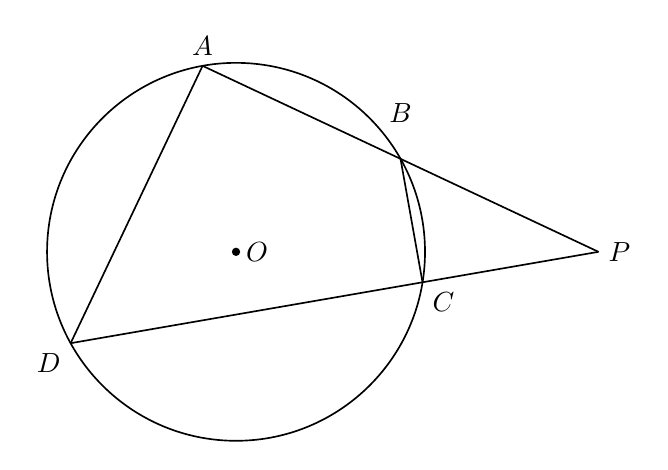
\begin{tikzpicture}[x=1cm,y=1cm,line width=.6pt,font=\normalsize]
% 圆 O 半径 2.4；A,B,C,D 在圆上，P 在圆外，A,B,P 共线（PB/PA=1/2），D,C,P 共线（PC/PD=1/3）
\coordinate (O) at (0,0);
\coordinate (A) at (-0.42480,2.36174);
\coordinate (B) at (2.08901,1.18099);
\coordinate (C) at (2.36844,-0.38686);
\coordinate (D) at (-2.10060,-1.16045);
\coordinate (P) at (4.60320,0);
\draw (O) circle[radius=2.4cm];
\draw (A)--(P);
\draw (D)--(P);
\draw (B)--(C);
\draw (D)--(A);
\fill (O) circle (1.5pt);
\node[right]      at (O) {$O$};
\node[above]      at (A) {$A$};
\node at (2.089,1.76) {$B$};
\node[below right] at (C) {$C$};
\node[below left] at (D) {$D$};
\node[right]      at (P) {$P$};
\end{tikzpicture}
